\chapter{Metodi del sottospazio di Krylov}
\subsection{Contesto generale}
Nel contesto della risoluzione di sistemi lineari derivanti da equazioni differenziali alle derivate parziali (PDE) discretizzate:
\begin{itemize}
	\item Le matrici dei coefficienti sono \textbf{sparse} (ad esempio, equazioni a 3, 5 o 7 punti).
	\item I metodi diretti, come la fattorizzazione LU, possono generare un \textbf{fill-in} significativo.
	\item La risoluzione di sistemi triangolari (es. $\mathbf{L}\mathbf{\psi} = \mathbf{b}$; $\mathbf{U}\mathbf{\phi} = \mathbf{\psi}$) può richiedere un numero eccessivo di FLOPs.
	\item Metodi come il \textbf{gradiente coniugato} (applicabile solo a matrici SPD) non aumentano il costo computazionale e la memoria con le iterazioni.
	\item L'estensione di questi metodi a matrici generali richiede la creazione di una base ortogonale incrementale per il \textbf{sottospazio di Krylov}.
	\item Tuttavia, il numero di FLOPs e la memoria crescono ad ogni iterazione.
\end{itemize}

\section{Sistema di equazioni lineari con matrice generale $\mathbf{A}$}
Dato il sistema di equazioni lineari:
\[
\mathbf{A} \mathbf{x} = \mathbf{b}, \quad \text{con } \mathbf{A} \in \mathbb{R}^{n \times n}, \mathbf{b} \in \mathbb{R}^{n}. 
\]
Dato un valore iniziale $\mathbf{x}_0$, si definisce il residuo $\mathbf{r}_0 = \mathbf{b} - \mathbf{A} \mathbf{x}_0$. La soluzione esatta può essere scritta come:
\[
\mathbf{x} = \mathbf{x}_0 + \mathbf{A}^{-1} \mathbf{r}_0. 
\]
\paragraph{Punto chiave:}
Poiché il calcolo di $\mathbf{A}^{-1}$ è spesso troppo costoso per sistemi sparsi di grandi dimensioni, è preferibile:
\begin{itemize}
	\item Cercare un'approssimazione di $\mathbf{A}^{-1} \mathbf{r}_0$;
	\item Utilizzare solo operazioni convenienti (ad esempio, prodotti matrice-vettore).
\end{itemize}

\section{Approssimazione di $\mathbf{A}^{-1}$}
Invece di calcolare $\mathbf{A}^{-1}$, si approssima la sua azione sul residuo $\mathbf{r}_0$ tramite un polinomio opportuno in $\mathbf{A}$:
\[
\mathbf{A}^{-1} \mathbf{r}_0\ \approx\ p_{k-1}(\mathbf{A}) \mathbf{r}_0\ =\ \sum_{i=0}^{k-1} c_i \mathbf{A}^i \mathbf{r}_0. 
\]
Quindi, una soluzione approssimata del sistema $\mathbf{A} \mathbf{x} = \mathbf{b}$ è:
\[
\mathbf{x}_k\ =\ \mathbf{x}_0\, +\, p_{k-1}(\mathbf{A}) \mathbf{r}_0\ \ . 
\]
\paragraph{Punto chiave:}
Ogni vettore della forma $p_{k-1}(\mathbf{A}) \mathbf{r}_0$ appartiene allo spazio:
\[
\mathcal{K}_k(\mathbf{A}, \mathbf{r}_0) = \operatorname{span}\{\mathbf{r}_0, \mathbf{A} \mathbf{r}_0, \dots, \mathbf{A}^{k-1} \mathbf{r}_0\}. \tag{5}
\]

\section{Il sottospazio di Krylov}

Lo spazio
\[
\mathcal{K}_k(\mathbf{A},\mathbf{r}_0)\ =\ \mathrm{span}\{\mathbf{r}_0,\,\mathbf{A}\mathbf{r}_0,\,\dots ,\,\mathbf{A}^{k - 1}\mathbf{r}_0\}
\]
è chiamato \textbf{sottospazio di Krylov} di ordine $k$.

\subsection{Interpretazione}
Cosa rappresentano gli elementi del sottospazio di Krylov? Immaginiamo $\mathbf{A}$ come l'approssimazione di un operatore differenziale:
\begin{itemize}
	\item $\mathbf{r}_0$: residuo iniziale;
	\item $\mathbf{A}\mathbf{r}_0$: misura della derivata (locale) del residuo;
	\item $\mathbf{A}^2\mathbf{r}_0, \ldots$: rappresentano derivate di ordine superiore (locali).
\end{itemize}
Ogni moltiplicazione per $\mathbf{A}$ estrae nuove informazioni sul comportamento del sistema.

\subsection{Forma del residuo}
Secondo l'equazione della soluzione approssimata di cui sopra, il residuo $\mathbf{r}_k$ assume la forma:
\[
\begin{aligned}
	\mathbf{r}_k\ &=\ \mathbf{b} - \mathbf{A} \mathbf{x}_k\ =\ \mathbf{b} - \mathbf{A} \left(\mathbf{x}_0 + p_{k-1}(\mathbf{A}) \mathbf{r}_0\right)\ = \\
	=\ \left(\mathbf{I} - \mathbf{A} p_{k-1}(\mathbf{A})\right) \mathbf{r}_0\ \ , 
\end{aligned}
\]
che, introducendo un nuovo polinomio matriciale di ordine $k$, $q_k(\mathbf{A}) = \left(\mathbf{I} - \mathbf{A} p_{k-1}(\mathbf{A})\right)$, si riduce a:
\[
\mathbf{r}_k = q_k(\mathbf{A}) \mathbf{r}_0\ \ . 
\]
La convergenza è quindi governata dalla capacità del polinomio matriciale $q_k(\mathbf{A})$ di smorzare efficacemente il residuo iniziale $\mathbf{r}_0$.

\subsection{Metodo di Krylov}
Un metodo di Krylov combina:
\begin{itemize}
	\item Uno spazio di ricerca per il vettore soluzione:
	\[
	\mathbf{x}_0 + \mathcal{K}_k(\mathbf{A}, \mathbf{r}_0); \tag{9}
	\]
	\item Un vincolo sul residuo.
\end{itemize}
Pwe quest'ultimo due scelte classiche sono:
\begin{itemize}
	\item \textbf{Condizione di Galerkin}:
	\[
	\mathbf{r}_k \perp \mathcal{K}_k(\mathbf{A}, \mathbf{r}_0); \tag{10}
	\]
	\item \textbf{Condizione di residuo minimo}:
	\[
	\left\| \mathbf{r}_k \right\|_2 = \min_{\mathbf{x} \in \mathbf{x}_0 + \mathcal{K}_k(\mathbf{A}, \mathbf{r}_0)} \left\| \mathbf{b} - \mathbf{A} \mathbf{x} \right\|_2. \tag{11}
	\]
\end{itemize}
Il metodo \textbf{GMRES} (Generalized Minimal RESidual) appartiene alla seconda classe.

%
%
%
\section{Da Conjugate Gradients a GMRES}
\subsection{Idea comune}
L'idea comune è costruire un'approssimazione della soluzione in un sottospazio di Krylov.

\subsubsection{Conjugate Gradients (CG)}
\begin{itemize}
	\item Applicabile solo a matrici \textbf{SPD} (Simmetriche e Definite Positive);
	\item Utilizza direzioni di ricerca \textbf{A-ortogonali};
	\item Minimizza l'errore nella norma di $\mathbf{A}$;
	\item Il costo computazionale è costante.
\end{itemize}

\subsubsection{GMRES}
\begin{itemize}
	\item Estende i metodi di Krylov a matrici generali;
	\item Richiede una base ortonormale (metodo di Arnoldi);
	\item Minimizza il residuo reale;
	\item Il costo computazionale cresce con le iterazioni.
\end{itemize}

\subsubsection{Regola pratica}
Il metodo CG è ottimale quando applicabile; GMRES viene utilizzato quando CG non può essere applicato.

%
%
\section{Metodo Generalized Minimal RESidual (GMRES)}

Dato un valore iniziale $\mathbf{x}_0$, all'iterazione $k$-esima l'approssimazione $\mathbf{x}_k$ è il vettore, nello spazio affine di Krylov $\mathbf{x}_0 + \mathcal{K}_k(\mathbf{A},\mathbf{r}_0)$, che minimizza la norma euclidea del residuo:
\[
\left\| \mathbf{r}_k \right\|_2 = \min_{\mathbf{x} \in \mathbf{x}_0 + \mathcal{K}_k(\mathbf{A}, \mathbf{r}_0)} \left\| \mathbf{b} - \mathbf{A} \mathbf{x} \right\|_2, \quad \mathbf{r}_0 = \mathbf{b} - \mathbf{A} \mathbf{x}_0. 
\]
Sviluppato originariamente da Y. Saad e M.H. Schultz (SIAM J. SCI. STAT. COMPUT., Vol. 7, No. 3, Luglio 1986).

\section{Metodo di Arnoldi}
Il metodo di Arnoldi costruisce incrementalmente una base ortonormale di $\mathcal{K}_k(\mathbf{A},\mathbf{r}_0)$:
\begin{itemize}
	\item Al passo $k$ produce un insieme $\mathbf{V}_k = [\mathbf{v}_1, \ldots, \mathbf{v}_k]$, con
	\[
	\mathbf{v}_i \cdot \mathbf{v}_j\ =\ \begin{cases}
		0, & \forall\ i \neq j \\
		1, & \text{se }\ i = j
	\end{cases} \qquad \text{con } i, j \in [1, \dots, k]\ \ , 
	\]
	tale che
	\[
	\operatorname{span}(\mathbf{r}_0, \mathbf{A} \mathbf{r}_0, \dots, \mathbf{A}^{k-1} \mathbf{r}_0) = \operatorname{span}(\mathbf{v}_1, \mathbf{v}_2, \dots, \mathbf{v}_k)\ \ .
	\]
\end{itemize}

\subsection{Procedura}
Partendo da $\mathbf{v}_1 = \frac{\mathbf{r}_0}{\|\mathbf{r}_0\|_2}$, in modo che $\|\mathbf v_1\|_2=1$ per $k = 1, 2, \ldots$:
\begin{enumerate}
	\item Calcolare: $\mathbf{w}_k = \mathbf{A}\mathbf{v}_k$;
	\item Ortogonalizzare rispetto alla base corrente:
	\[
	\text{per } i = 1, 2, \dots, k: \quad h_{ik} = (\mathbf{w}_k, \mathbf{v}_i), \tag{15}
	\]
	\[
	\hat{\mathbf{v}}_{k+1} = \mathbf{w}_k - \sum_{i=1}^{k} h_{ik} \mathbf{v}_i; \tag{16}
	\]
	\item Porre $h_{k+1,k} = \|\hat{\mathbf{v}}_{k+1}\|_2$;
	\item Se $h_{k+1,k} = 0$ $\rightarrow$  FERMARSI (la base è completa);
	\item Altrimenti, normalizzare il nuovo vettore:
	\[
	\mathbf{v}_{k+1} = \frac{\hat{\mathbf{v}}_{k+1}}{h_{k+1,k}}. \tag{17}
	\]
\end{enumerate}

\[
\begin{aligned}
	h_{11}\ &=\ (\mathbf w_1,\,\mathbf v_1)\ =\\
	&=\ |\mathbf w_1|\, |\mathbf v_1|\, \cos(\alpha)\ =\\
	&=\ |\mathbf w_1|\, \cos(\alpha)
\end{aligned}
\qquad \qquad
\begin{aligned}
	\hat{\mathbf v}_2\ &=\ \mathbf w_1\, h_{11} \mathbf v_1|\ =\\
	&=\ |\mathbf w_1|\, +\, (-h_{11}\mathbf v_1)
\end{aligned}
\]

\begin{figure}[h]
	\centering
	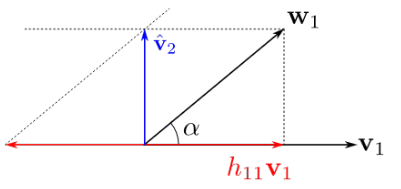
\includegraphics[width=0.5\textwidth]{img/Arnoldi_matrix.png}
	\caption{Visualizzazione del primo step del processo di ortogonalizzazione di Arnoldi.}
	\label{fig:arnoldi_process}
\end{figure}


\subsection{Forma matriciale}
Combinando le formule riportate nella procedura, si ottiene:
\[
h_{k+1,k} \mathbf{v}_{k+1}\ =\ \mathbf{A} \mathbf{v}_k\, -\, \sum_{i=1}^{k} h_{ik} \mathbf{v}_i\ \ , 
\]
e quindi:
\[
\mathbf{A} \mathbf{v}_k\ =\ \sum_{i=1}^{k} h_{ik} \mathbf{v}_i\, +\, h_{k+1,k} \mathbf{v}_{k+1}\ =\ \sum_{i=1}^{k+1} h_{ik} \mathbf{v}_i\ \ . 
\]

\[
\begin{aligned}
	\mathbf{A} \mathbf{v}_1\ &=\ h_{11} \mathbf{v}_1 + h_{21} \mathbf{v}_2\\
	\mathbf{A} \mathbf{v}_2\ &=\ h_{12} \mathbf{v}_1 + h_{22} \mathbf{v}_2 + h_{32} \mathbf{v}_3 \\
	&\vdots \\
	\mathbf{A} \mathbf{v}_k\ &=\ h_{1k} \mathbf{v}_1 + h_{2k} \mathbf{v}_2 + \dots + h_{k+1,k} \mathbf{v}_{k+1}\\
\end{aligned}
\]

In forma matriciale, si ha:
\[
\mathbf{A V}_k = \mathbf{V}_{k+1} \bar{\mathbf{H}}_k\ \ , 
\]
dove $\bar{\mathbf{H}}_k$ è una \underline{matrice di Hessenberg superiore} (con zeri sotto la prima sottodiagonale) e $\mathbf{V}_l$ (con $l = k, k+1$) è una matrice le cui colonne sono i vettori $\mathbf{v}_i$ con $i = 1, \dots, l$.

\begin{figure}[h]
	\centering
	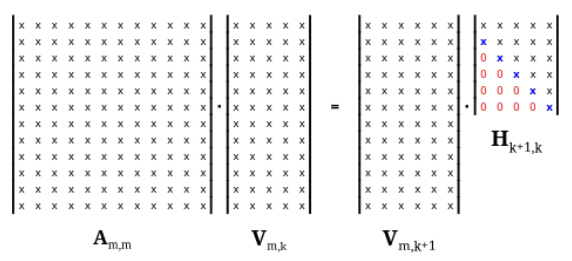
\includegraphics[width=0.6\textwidth]{img/Arnoldi_matrix2.png}
	\caption{Rappresentazione della forma matriciale.}
	\label{fig:arnoldi_matrix}
\end{figure}

%
%
\section{Metodo GMRES}

Il processo di Arnoldi descritto consente di riscrivere l'equazione iniziale nella forma:
\[
\mathbf{x}_k = \mathbf{x}_0 + \mathbf{V}_k \mathbf{y}, \qquad [\mathbf{x}_k,\ \mathbf{x}_0 \in \mathbb{R}^n;\ \mathbf{y} \in \mathbb{R}^k;\ \mathbf{V}_k \in \mathbb{R}^{n \times k}]\ \ . 
\]
Quindi, il residuo $\mathbf{r}_k$ diventa:
\[
\mathbf{r}_k\ =\ \mathbf{b} - \mathbf{A} \mathbf{x}_k\ =\ \mathbf{r}_0 - \mathbf{A} \mathbf{V}_k \mathbf{y}\ \ . 
\]
Grazie all'equazione di $\mathbf{A} \mathbf{V}_k$, si ottiene:
\[
\mathbf{r}_k\ =\ \mathbf{r}_0 - \mathbf{V}_{k+1} \bar{\mathbf{H}}_k \mathbf{y}, \quad [\mathbf{V}_{k+1} \in \mathbb{R}^{n \times (k+1)}; \bar{\mathbf{H}}_k \in \mathbb{R}^{(k+1) \times k}]\ \ . 
\]

\subsection{Minimizzazione del residuo}
Ponendo $\beta = \|\mathbf{r}_0\|_2$, si ha $\mathbf{v}_1 = \frac{\mathbf{r}_0}{\beta}$ e $\mathbf{r}_0 = \beta \mathbf{v}_1$. Ovviamente,
\[
\mathbf{v}_1\ =\ \mathbf{V}_{k+1}\, \mathbf{e}_1\ \ , 
\]
dove $\mathbf{e}_1$ è la prima colonna della matrice identità $\mathbf{I} \in \mathbb{R}^{(k+1) \times (k+1)}$. $\mathbf r_k$ può essere riscritta come:
\[
\mathbf{r}_k\ =\ \beta \mathbf{V}_{k+1} \mathbf{e}_1 - \mathbf{V}_{k+1} \bar{\mathbf{H}}_k \mathbf{y}\ =\ \mathbf{V}_{k+1}\, (\beta \mathbf{e}_1 - \bar{\mathbf{H}}_k \mathbf{y})\ \ .
\]
Poiché $\mathbf{V}_{k+1}$ è una matrice con colonne ortonormali, preserva la lunghezza dei vettori a cui è applicata. Quindi, dall'equazione precedente, si ottiene:
\[
\|\mathbf{r}_k\|_2\ =\ \|\beta \mathbf{e}_1 - \bar{\mathbf{H}}_k \mathbf{y}\|_2\ \ . 
\]

L'obiettivo di GMRES è minimizzare, a ogni passo, la norma del residuo $\mathbf{r}_k$, cioè trovare il vettore $\mathbf{y}_k$ tale che:
\[
\mathbf{y}_k\ =\ \text{arg}\min_{\mathbf{y} \in \mathbb{R}^k}\, \|\beta \mathbf{e}_1 - \bar{\mathbf{H}}_k \mathbf{y}\|_2\ \ . 
\]
In conclusione, il grande sistema lineare sparso $\mathbf{A}\mathbf{x} = \mathbf{b}$ (con $n$ equazioni e $n$ incognite) è ridotto a successivi problemi di minimi quadrati (con $k+1$ equazioni e $k$ incognite) di ordine crescente $k$.
Se la convergenza è raggiunta dopo $k^*$ step ($\|\mathbf{r}_{k^*}\|_2 <\epsilon $), la soluzione sarà $\mathbf{k^*}\ =\ \mathbf{x}_0 + \mathbf{V}_{k^*} \mathbf{y}_{k^*}$.
%
%
%
\begin{lstlisting}[caption={Algoritmo GMRES}]
r_0 =  b  -  A * x_0;
beta =  ||r0||_2; 
v_1 =  r0  /  beta;
FOR k = 1, ..., k DO:
	w = A * vk;
	FOR i = 1, ..., k DO:
		h_ik = v_i^T * w;
		w -=  h_ik * v_i$;
	h_{k+1,k} = ||w||_2;
	IF h_{k+1,k} = 0 THEN
		 FERMARSI (lucky breakdown!);
	END IF	
	v_{k+1} =  w  /  h_{k+1,k};
	risolvere il problema ai minimi quadrati: min ||beta e_1 - H_k y||_2;
	
	IF ||r||_2 < \epsilon THEN
		 uscire dal ciclo for;
	END IF
END FOR
x_k =  x_0  +  V_k * y_k
\end{lstlisting}
%
%
%
\section{GMRES con Riavvio (Restarted GMRES)}

Aumentare $k$ richiede:
\begin{itemize}
	\item Maggiore memoria per immagazzinare i vettori della base ortonormale;
	\item Tempo di calcolo più lungo per eseguire l'ortogonalizzazione completa;
	\item Risolvere problemi ai minimi quadrati di ordine crescente $k$.
\end{itemize}
In aritmetica esatta, GMRES converge alla soluzione esatta in al più $n$ passi, ma il costo computazionale cresce a livelli inaccettabili.

\subsubsection{Strategia di riavvio}
Si adotta la seguente strategia, nota come \textbf{GMRES($k_0$)}:
\begin{itemize}
	\item Scegliere un intero fisso $k_0$;
	\item Se la convergenza non viene raggiunta in al più $k_0$ passi, calcolare $\mathbf{x}_{k_0}$;
	\item Riavviare il processo utilizzando $\mathbf{x}_{k_0}$ come nuova ipotesi iniziale.
\end{itemize}

\subsubsection{Vantaggi}
\begin{itemize}
	\item Memoria limitata;
	\item Costo di ortogonalizzazione limitato.
\end{itemize}

\subsubsection{Possibili svantaggi}
\begin{itemize}
	\item Convergenza più lenta o stagnazione a causa della perdita di informazioni spettrali accumulate durante i passi precedenti.
\end{itemize}

\subsubsection{Compromesso}
Un valore di riavvio più grande, $k_0$, generalmente migliora la convergenza, ma aumenta la memoria e il costo per passo.

\subsubsection{Takeaways}
\begin{itemize}
	\item Il GMRES completo è spesso più robusto;
	\item Il GMRES con riavvio è più pratico per problemi su larga scala.
\end{itemize}

%
%
%
\section{Precondizionamento}

In pratica, i metodi di Krylov vengono raramente utilizzati senza precondizionamento.

L'obiettivo del precondizionamento è sostituire il sistema originale con uno equivalente che abbia migliori proprietà numeriche per l'iterazione.

%
%
\subsection{Scelte comuni}
\begin{itemize}
	\item \textbf{Precondizionamento a sinistra}: $\mathbf{M}^{-1}\mathbf{A}\mathbf{x} = \mathbf{M}^{-1}\mathbf{b}$;
	\item \textbf{Precondizionamento a destra}: $\mathbf{A}\mathbf{M}^{-1}\mathbf{y} = \mathbf{b}$, $\mathbf{x} = \mathbf{M}^{-1}\mathbf{y}$.
\end{itemize}

La matrice $\mathbf{M}^{-1}$ dovrebbe:
\begin{itemize}
	\item Essere una buona approssimazione di $\mathbf{A}^{-1}$;
	\item Produrre un nuovo operatore con autovalori più raggruppati e lontani dall'origine;
	\item Essere economica da applicare.
\end{itemize}

%
%
\subsection{Differenze tra precondizionamento a sinistra e a destra}

Precondizionamento a sinistra
\begin{itemize}
	\item Dalla definizione di cui sopra: $\tilde{\mathbf{r}}_0 = \mathbf{M}^{-1}(\mathbf{b} - \mathbf{A}\mathbf{x}_0) = \mathbf{M}^{-1}\mathbf{r}_0$;
	\item Il processo minimizza un residuo diverso, che potrebbe non riflettere accuratamente l'errore della soluzione reale.
\end{itemize}

Precondizionamento a destra:
\begin{itemize}
	\item Introduce il cambio di variabile $\mathbf{x} = \mathbf{M}^{-1}\mathbf{y}$;
	\item Dalla definizione di cui sopra: $\tilde{\mathbf{r}}_0 = \mathbf{b} - \mathbf{A}\mathbf{M}^{-1}\mathbf{y}_0$, ma essendo $\mathbf{y}_0 = \mathbf{M}\mathbf{x}_0$, si ha $\tilde{\mathbf{r}}_0 \equiv \mathbf{r}_0$;
	\item Il processo minimizza il residuo corretto, permettendo di tenere sotto controllo l'errore della soluzione reale;
	\item Ottenuta la soluzione $\mathbf{y}$, è necessario risolvere il problema aggiuntivo $\mathbf{M}\mathbf{x} = \mathbf{y}$ per ottenere $\mathbf{x}$.
\end{itemize}

\subsection{Esempi di precondizionamento}
\subsubsection{Precondizionamento di Jacobi}
\begin{itemize}
	\item $\mathbf{M} = \mathrm{diag}(\mathbf{A})$;
	\item È il più semplice;
	\item Guadagno limitato;
	\item Adatto per matrici $\mathbf{A}$ diagonalmente dominanti;
	\item Avvicina $\mathbf{A}$ alla matrice identità.
\end{itemize}

\subsubsection{Fattorizzazione LU incompleta (ILU)}
\begin{itemize}
	\item Trova $\mathbf{M} = \tilde{\mathbf{L}}\tilde{\mathbf{U}} \approx \mathbf{A}$;
	\item La versione senza fill-in, ILU(0), forza a rimanere zero gli elementi che sono già zero in $\mathbf{A}$ (sebbene in una fattorizzazione LU completa non lo sarebbero);
	\item Originariamente ideata per le matrici a 5 e 7 punti derivanti dalla discretizzazione di PDE ellittiche per problemi 2D e 3D.
\end{itemize}